\chapter{The First Chapter}

This is the first chapter. It contains a lot of text. Footnotes can also be
used\footnote{This is a footnote}. Remember to format the
URLs\footnote{\url{http://www.example.com}}. For adding a citation in
parentheses, use the \emph{citep} command \citep{dummy1}. If you need to refer
to the name of the author, use the \emph{cite} command, for example when talking
about the esteemed \cite{dummy2}.

\section{Figures and Tables}

When referring to figures, use the \emph{ref} command. This ensures numbering
will stay correct when adding or removing sections. For example, let's talk
about Figure~\ref{figure:example}. Then, let's mention
Table~\ref{table:example}.

\section{Another Section}

Lorem ipsum dolor sit amet, consectetur adipiscing elit. Sed quis tempus ipsum.
Nulla ornare velit sit amet lectus aliquam, eget elementum diam faucibus.
Phasellus scelerisque elit non leo fringilla, non dictum risus eleifend. Morbi
suscipit eleifend augue ut vehicula. Proin at dolor tincidunt arcu convallis
vestibulum vitae eget erat. Quisque a quam libero. Donec scelerisque, nisl in
consectetur rhoncus, dolor ex vestibulum ante, non porttitor nisi tellus eget
nulla. Ut maximus vitae neque vel porta. Morbi suscipit tristique leo vitae
aliquam. Nullam congue malesuada scelerisque. Sed viverra ipsum id quam tempor,
eget posuere lacus fringilla. Suspendisse sit amet orci augue. Aliquam tincidunt
volutpat purus scelerisque sollicitudin. Fusce eleifend porttitor velit
tincidunt commodo. Etiam rhoncus nunc eget sapien pretium, vitae blandit tortor
elementum. Nam placerat eu metus ut ultrices.

\begin{figure}[!tpb]
\centerline{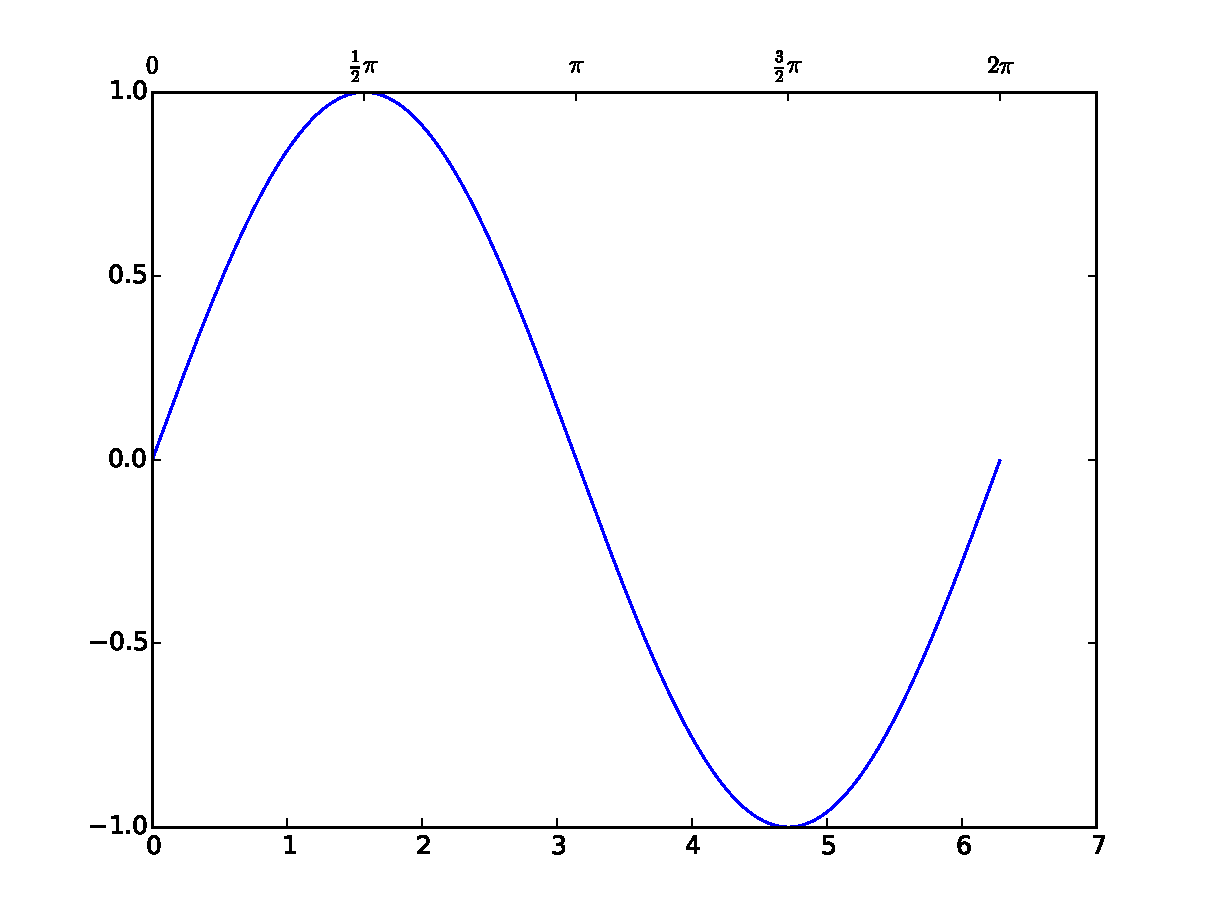
\includegraphics[width=0.5\textwidth]{figures/example.pdf}}
\caption{This is a caption. Example figure made with matplotlib
(\url{http://matplotlib.org}).}
\label{figure:example}
\end{figure}

\begin{table}[t!]
\centering
{\small
\begin{tabular}{l|r|r}
Key & Value & Index  \\
\hline
Example A & 100 & 1 \\
Example B & 1000 & 2 \\
Example C & 5 & 3  \\
\hline
\end{tabular}}
\caption{This is a caption.}
\label{table:example}
\end{table}